\section{Introduction}
\label{sec:intro}

Strong public representations have changed where the cost of a classifier
lies. A frozen vision or text encoder already places semantically similar
records near each other, so a data platform can expose class structure
before it owns a single task label. What remains scarce is
\emph{supervision}: public annotation, at a cost and under acquisition rights
that determine which examples may be requested, or private clients, such as
devices, organizations or user accounts, whose labelled records are reachable
only through protected aggregate interfaces.

A platform that wants to publish a classifier therefore makes three decisions
(Figure~\ref{fig:scenario}): \emph{what supervision to buy}, public labels or
private reports; \emph{what statistic to release} from clients, per-example
votes, a compact regional summary or a clipped model head; and \emph{what
evidence to require} before publication. Evaluated separately and judged by average
accuracy, reported gains mix these resources and do not transfer.

% Schematic (no data): the platform's three decisions (vector figure, experiments/release-eab9-20261021/figure-source).
\begin{figure}[t]
\centering
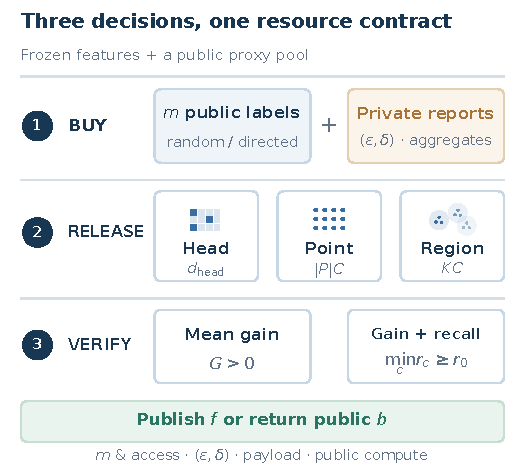
\includegraphics[width=.92\columnwidth,trim=0 .02in 0 .56in,clip]{figures/fig-decision-map.pdf}
\Description{Three platform decisions: buy public labels and/or private
reports, choose a release object (head, point or region), and choose the
verification target before publishing a candidate or the public comparator.}
\caption{Three platform decisions under a shared resource contract: the
acquisition contract for public labels and private supervision, the
protected release object, and the evidence required before publication.}
\label{fig:scenario}
\end{figure}


\subsection{An experiment and analysis study}

This paper is an experimental analysis, not a new release mechanism:
regional naming, distributed discrete-Gaussian aggregation and noisy-count
confidence bounds are established components. Its contribution is a
\emph{resource-matched evaluation protocol} and what it reveals. The
protocol measures private value against the strongest public learner with the
same labels, representation and acquisition mode (Section~\ref{sec:problem});
every comparison fixes annotation budget and acquisition mode, total
whole-client privacy budget, released coordinates and public post-processing,
and verification is charged to the same total budget as naming. We apply it
to 3426 inherited primary records over 90 cohorts and 4224 public label sets,
and to five studies whose designs were frozen before they ran
(Table~\ref{tab:studies}). Image clients are simulated privacy units built
from public benchmarks; Usenet authors and FEMNIST writers are natural.

\subsection{Findings}

\paragraph{Finding 1: acquisition rights decide private value}
With ten random CIFAR-1k labels at $(\varepsilon,\delta)=(.1,10^{-5})$, joint
naming beats the strongest of fourteen equal-budget public learners by
\JointGain{} points on average (median \GainMedian{}), though
\GainNegativeDraws{}\% of label draws lose. Ten feature-directed labels
recover the same \CeilCifar{}\% classifier without private reports: an
evaluation must fix both how many labels exist and how they are acquired.
With a weaker ResNet-18 encoder, directed labels again reach the partition
ceiling without private reports, but random-label joint naming changes the
strongest public learner by \EncGain{} points: passive private value also
needs regions that carry the classes.

\paragraph{Finding 2: raw sensitivity does not rank release interfaces}
Per-example votes on $|P|=2000$ proxy points are $\sqrt{|P|/K}\approx14$
times more sensitive than a $K=10$ regional report and need 20000 rather than
100 coordinates. Yet averaging point votes inside each region brings their
noise to .88--1.07 times the regional level, and pooled point and regional
joint naming differ by at most \PointRegionMaxGap{} points on all
\PointRegionSettings{} tested settings. The protected head, a different
object, wins where the partition limits regional naming (MNIST:
\HeadMnistTenK{} versus \RegionMnistTenK{}\%). Payload and partition fit, not
sensitivity, should choose the interface.

\paragraph{Finding 3: publication evidence is a separate resource}
On held-out clients charged to one total budget, a mean-gain certificate is
cheap, accepting \MiddleGlobalAccept{}\% of cases at $\varepsilon=1$, but
\MinRecGainOneTenth{}\% of the classifiers it publishes recall some test class
below $10\%$. Class evidence costs more, at a price set by the protocol. A naming share selected on independent
development cohorts, frozen, and confirmed on new cohorts and the test split
raises all-class acceptance from \BCFixedRecallOne{}\% to
\BCFrozenRecallOne{}\% at $\varepsilon=1$ ($\BCDiffRecallOneUtil$ test
accuracy points), makes recall $\ge.5$ certifiable at $\varepsilon=3$
(\BCFrozenHalfThree{}\%), leaves mean-gain release unchanged and records no
false accept. On natural FEMNIST writers, where no class target is reachable,
a calculator prediction frozen before confirmation lands within \FCPlanGap{}
points in every cell, and \FCTail{}\% of the classifiers the mean-gain rule
publishes recall some class below 10\%.

\paragraph{Explaining the losses}
Stored noise-free votes split the gap below the partition ceiling into signed
differences: teacher content dominates on Usenet, release noise on CIFAR-1k
and FEMNIST at $\varepsilon=.1$, selection on MNIST and CIFAR-10k. Private
verification of a noise-gated rule screens cases, not tasks.

\subsection{Contributions}
\begin{itemize}[leftmargin=*,itemsep=1pt,topsep=2pt]
\item A resource-matched evaluation protocol with annotation access, privacy
budget, payload and publication target as separate resources
(Section~\ref{sec:problem}), and a map of which information supports
deployment decisions (Section~\ref{sec:discussion}).
\item Three findings on what to buy, release and verify, with a weaker-encoder
ablation, published per-example and head baselines on the same protected sum,
a cost ladder, tighter-band and source-disjoint controls, a budget split
selected on independent cohorts and confirmed on CIFAR, and a
Gaussian-approximation acceptance calculator tested on natural FEMNIST writers
(Sections~\ref{sec:eval:main}--\ref{sec:eval:verification}).
\item Signed differences below a decoder-matched partition ceiling that
locate the loss on four tasks, and a pre-registered study of gated selection
plus verification (Section~\ref{sec:eval:ceiling}).
\item A public artifact that regenerates every number from immutable records
and replays protected outputs from retrained cohorts.
\end{itemize}
